\documentclass[9pt,twocolumn,twoside,lineno]{pnas-new}

\templatetype{pnasresearcharticle}
\graphicspath{{../figures/}}

\title{Deconstructing the gender gap in chess ratings}

\author[a,1,2]{Wei Ji Ma}
\author[b,1]{Nikos I. Bosse}
\author[c,1]{Jose Camacho-Collados}
\author[d,1]{Richard L. Smith}
\author[e,1]{Gy\"orgy Barab\'as}
\author[f]{David Smerdon}
\author[g]{Yifan Hou}

\affil[a]{Center for Neural Science and Department of Psychology, New York University}
\affil[b]{London School of Hygiene and Tropical Medicine}
\affil[c]{School of Computer Science and Informatics, Cardiff University}
\affil[d]{Department of Statistics and Operations Research, University of North Carolina}
\affil[e]{Department of Physics, Chemistry and Biology, Link\"oping University}
\affil[f]{School of Economics, University of Queensland}
\affil[g]{School of Physical Education, Shenzhen University; four-time Women's World Chess Champion}
\leadauthor{Ma}

\significancestatement{There is a lot of public discourse about gender differences in chess ability. While we can use FIDE ratings to measure ability, the gaps in ratings seen between top men and women are statistically confounded by differences in participation rate, experience level, and age. Here, we control for those differences and calculate the remaining gender gap in three metrics at the level of national federations. While a gap remains, it is much smaller than the raw data indicate. We test the robustness of our results against changes in the data filter.}

\authorcontributions{All authors intellectually developed the work, designed analyses, and contributed to the writing of the manuscript. W.J.M., N.I.B., J.C.C., R.L.S., and G.B. performed statistical analyses.}
\authordeclaration{No competing interests.}
\equalauthors{\textsuperscript{1}Authors W.J.M., N.I.B., J.C.C., D.S., and R.L.S. contributed equally to this work.}
\correspondingauthor{\textsuperscript{2}To whom correspondence should be addressed. E-mail: weijima@nyu.edu}

%At least three keywords are required at submission. Please provide three to five keywords, separated by the pipe symbol.
\keywords{gender differences $|$ chess $|$ ratings $|$ ability beliefs}

\begin{abstract}
In most federations, there is a difference in performance between top man and woman chess players, which we will call the {\it top-level gap}. The origins of this gap have been widely debated, with popular discourse often focusing on biological, social and cultural explanations. It has been noted before that a top-level gap is expected given the {\it participation gap} -- the fact that only 10\% of rated chess players are women. In the first part of this work, we ask to what extent, in individual federations, the top-level gap can be accounted for by the participation gap. We use ratings of the World Chess federation as an objective measure of performance. Using permutation tests, we find that the proportion explained is XX$\pm$YY\% for the top 1 male and women, and XX$\pm$YY\% for the average of the top 10. Beyond the top players, we find a significant gender gap in the average rating of all active players in XX out of YY federations. Examining the so-called male variability hypothesis, we find/do not find a gender difference in the standard deviation. In the second part of this work, we do a comprehensive inventory of social, cultural,  economic, and biological factors that could contribute to (1) the part of the top-level gap not accounted for by the participation gap; (2) the participation gap itself. Some of these factors have so far only been anecdotally reported  and further research into their validity and their impact is needed.

\end{abstract}

\dates{This manuscript was compiled on \today}
\doi{\url{www.pnas.org/cgi/doi/10.1073/pnas.XXXXXXXXXX}}


%Todo: check Barry Hyman: https://www.chessable.com/blog/gender-gap-chess/
% Larry Cahill

\begin{document}

\maketitle
\thispagestyle{firststyle}
\ifthenelse{\boolean{shortarticle}}{\ifthenelse{\boolean{singlecolumn}}{\abscontentformatted}{\abscontent}}{}

In most federations, the strongest male chess player has a higher rating than the strongest female chess player. We refer to this difference as the {\it top gap}, and in this paper, we try to  characterize the top gap and  understand how it comes about. We will use a variety of methods. We will use statistical analysis to establish to what extent the top gap in a given federation is due to confounding factors such as a participation gap, a difference in age, or a difference in experience. After correcting for those factors, we will explore whether any federation-level indicators predict the residual top gap. Next, we turn to the literature on gender stereotypes and gender biases to do an inventory of the factors known from other domains that might affect any residual gap. Arguments in this section will generally apply not only to the top gap but to players of all levels. Finally, we will take an anthropological view and discuss the first-person experiences of one of us, a Women's World Champion.

\subsection*{The participation rate hypothesis}
Chess players are commonly rated according to the ELO rating system \cite{elo}, which assigns each player a number based on the strength of their opponents and their record of wins, draws and  losses in rated competitions. Ratings are published each month by the International Chess federation (commonly known by its French acronym, FIDE); in addition, leading chess federations, such as those of
the USA and Germany, maintain their own national rating lists. Although the rating list does not  discriminate between male and women, it has been a persistent phenomenon since the earliest days of this system that men by far dominate the top places in the rating system.

\cite{charness1996participation} were apparently the first authors to suggest that the discrepancy between male and female ratings could be explained by the differences in numbers of participants, which we henceforth refer to as the {\it participation rate hypothesis}. Using statistical formulas for the
distributions of extreme values in large samples, they pointed out that for many (though not all) statistical distributions, the maximum of a sample of size $n$ grows as a linear function in log $n$, and used this to examine not only the male-female discrepancy but also the predominance of certain
federations (in particular, Russia) among the top players. They concluded that
``the expected differences [according to the log-linear relationship] are very close to the observed
differences." However, they noted the caveat that chess ratings are not necessarily normally distributed,
an assumption that underlay their numerical results.

\cite{chabris2006sex} used US ratings to examine the relative performance of male and women in
different age ranges, concluding that \textit{the greater number of men at the highest levels in chess
can be explained by the greater number of boys who enter chess at the lowest levels}. As part of their
study, they noted that the mean male-female rating difference decreased when plotted against the overall percentage of women in a sample of 6-12 year old players across approximately 60 US zipcodes,
a finding that supports the participation rate hypothesis.

\cite{bilalic2009best} noted that a weakness of the method of \cite{charness1996participation} was their
focus on the top player alone, which is subject to a lot of variability. Using standard formulas for
expectations of order statistics \cite{davidnagaraja}, they used German rating data to study male-female
rating differences among the top 100 players, and concluded that
\textit{96 per cent of the observed difference would be expected given the much greater number of men who play chess}. However, they again assumed the underlying distribution of ratings is normal, which is
not necessarily correct.

Knapp \cite{knapp2010prsb} pointed out this weakness and proposed an alternative method based on the \textit{hypergeometric distribution}. Given the total numbers of male and women in a population, the hypergeometric distribution allows us to answer questions of the form ``what is the distribution of the number of women among the top 100 (or some other number) of players in the population?"
This assumes only that the distribution of male and female ratings is the same without making any assumption that it has a normal or some other specified distribution. However, Knapp's method does not directly address the numerical difference in ratings between top male and women.

Other authors have disputed these findings. For example, \cite{howard2014jbs} argued for need to correct
for differences in age and experience and advanced an alternative ``natural talent" hypothesis.

Other authors have critiqued these studies from different points of view, for example, suggesting
that the statistical approximations used were inadequate \cite{wiesend}.
However, none has provided a formal statistical test of the participation rate hypothesis. A major
purpose of the present article is to propose such a test.

\section*{Methods}
\subsection*{Data source}
We use Elo ratings as the most  widely used measure of chess performance available, while we have to keep in mind that the reliability of a rating depends on the number and recency of games played.
We prefer FIDE ratings over national ratings because it will allow us to compare federations on a more even footing. We choose standard ratings because they are based on the largest number of games, and because the largest number of players have a standard rating.


FIDE publishes a new rating list every month. We use the December 2019 rating list because the COVID-19 pandemic, which became widespread in January 2020, caused very few rated games to be played in 2020 and 2021.

We used the file downloaded on Jul 18, 2023


\cite{vacigulabilalic} criticized studies based on the FIDE rating list because it does not include all players in rated competitions. Originally, the FIDE list only included players rated 2200 or higher (national master standard). The threshold for inclusion was gradually lowered and now (as of 2021)  includes players down to a rating of 1000, which is effectively the standard of a beginner or a  casual player. \cite{vacigulabilalic} recommended using a national database (in their case, German) because the national database contains all players whereas the FIDE database contains only a subset. Their criticism may be less relevant given the expansion of the FIDE list in recent years, but the possibility that different federations may have different criteria for submitting results to FIDE may still be a possible source of bias.


\subsection*{Data filters}

There were 8749 individuals whose year of birth was unknown. As several of our analyses use age, or junior status, we excluded these individuals.

There were no individuals whose gender was reported as unknown.



In our main analyses, we {\it exclude} inactive players and {\it include} junior players, resulting in players from 187 federations. (We will examine the robustness of our results against these choices.) The resulting data set contains 172,843 players, of whom 155,368 were men and 17,389 were women (10.06\%). Fig. \ref{fig:summ_stats} shows the histograms of ratings of all men and all women. The male ratings range from 1001 to 2872 (Magnus Carlsen), whereas the female ratings range from 1001 to 2664 (author Hou Yifan). FIDE states that it removes players whose ratings drop below 1000 from the list; this removal seems to extend to players whose rating equals 1000.  For federation-by-federation analyses, we only include the 79  federations that have at least 30 FIDE-rated women. All of these federations also have at least 30 FIDE-rated men.





\subsection*{Statistical tests}
Our main tool to test for gender differences in summary statistics of FIDE ratings is a permutation test with 1 million samples. Not only does this test allow us to avoid specifying the parametric form of the rating distribution, it also works for summary statistics for which no good parametric test is available, such as the maximum rating. The reported $p$-value is two times the proportion of sampled differences smaller or larger than the observed difference, whichever is smaller. Thus, $p=0$ means that none of our simulations returned a value more extreme than the observed value.

One issue of concern in this type of analysis is \textit{multiple comparisons}. When the same test is applied simultaneously to multiple federations at the 0.05 significance level, it is inevitable that some of the tests will lead to rejection even if all the null hypotheses are true. Although there is no perfect answer to this, we shall apply one of the most common tools for correcting the $p$-values, the \textit{false discovery rate} (FDR) method of \cite{BH95}.

\section*{Results}


\subsection*{Distribution}
Before we turn to gender gaps in the top ratings, we first compare the ratings of men and women across all levels. A Wilcoxon-Mann-Whitney test revealed that the rating distributions of men and women are significantly different ($U_\mathrm{male} = 1779196335$, $p = 0$, $95\%$ confidence limits: $[215, \, 226]$). We next repeated this test at a federation level, focusing on the 79 federations that have at least 30 female FIDE-rated players in our data set. We found that the rating distributions of men and women are significantly different in 74 out of 79 federations (all except Azerbaijan, Bulgaria, Georgia, Kazakhstan, and Latvia). A Kolmogorov-Smirnov (KS) test on the 79 $p$-values revealed a distribution that was significantly different from uniform ($D = 0.90$, $p = 2.2 \times 10^{-16}$). We conclude that both at the world and at the federation level, the  rating distributions of men and women are different.

 \begin{figure}[!ht]
     \centering
     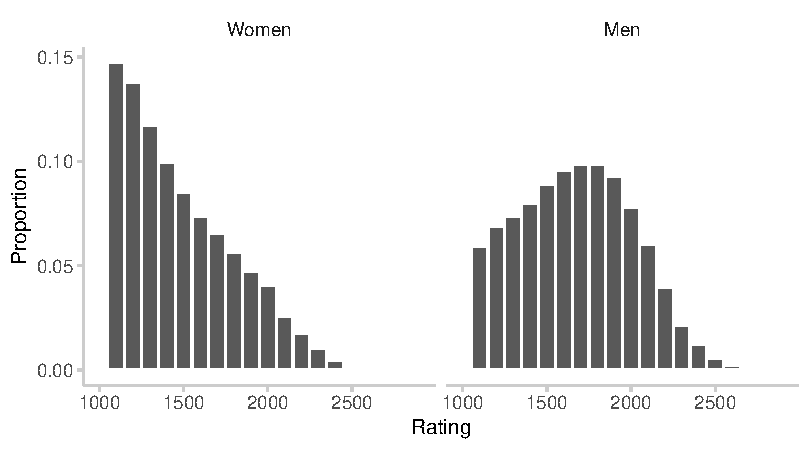
\includegraphics[width = \linewidth]{fig_1_w_jun_no_ina.pdf}
     \caption{Histograms of ratings of active women and men chess players across the world. We binned the data from 1000 to 2900 in bins of size 100. All data in this paper are from the December 2019 FIDE rating list. Our main analyses include junior players but exclude inactive players.}
     \label{fig:summ_stats}
 \end{figure}

\subsection*{Mean}
The mean rating of men was 1658.25, and of women 1451.53, for a difference of 206.72.  A permutation test revealed that this was significantly different from 0 with a $p$-value of 0.  We next analyzed mean ratings by federation (Fig. \ref{fig:federation-differences}A and Table \ref{tab:main_by_federation}). In all 79 federations, the mean for men was higher than for women. The difference was significant in 74  federations, the same ones as in the Wilcoxon-Mann-Whitney test above. A KS test on the $p$-values revealed a distribution that was significantly different from uniform ($D = 0.92$, $p < 2.2\times 10^{-16}$). To deal with the multiple-comparisons problem, we applied the False Discovery Rate correction \cite{BH95} to the $p$-values. We found that the number of statistically significant federations stayed at 74; the KS test again returned $D = 0.92$ ($p < 2.2\times 10^{-16}$). We conclude that in the vast majority of federations, men on average have a higher FIDE rating than women.
  \begin{figure}[!ht]
     \centering
     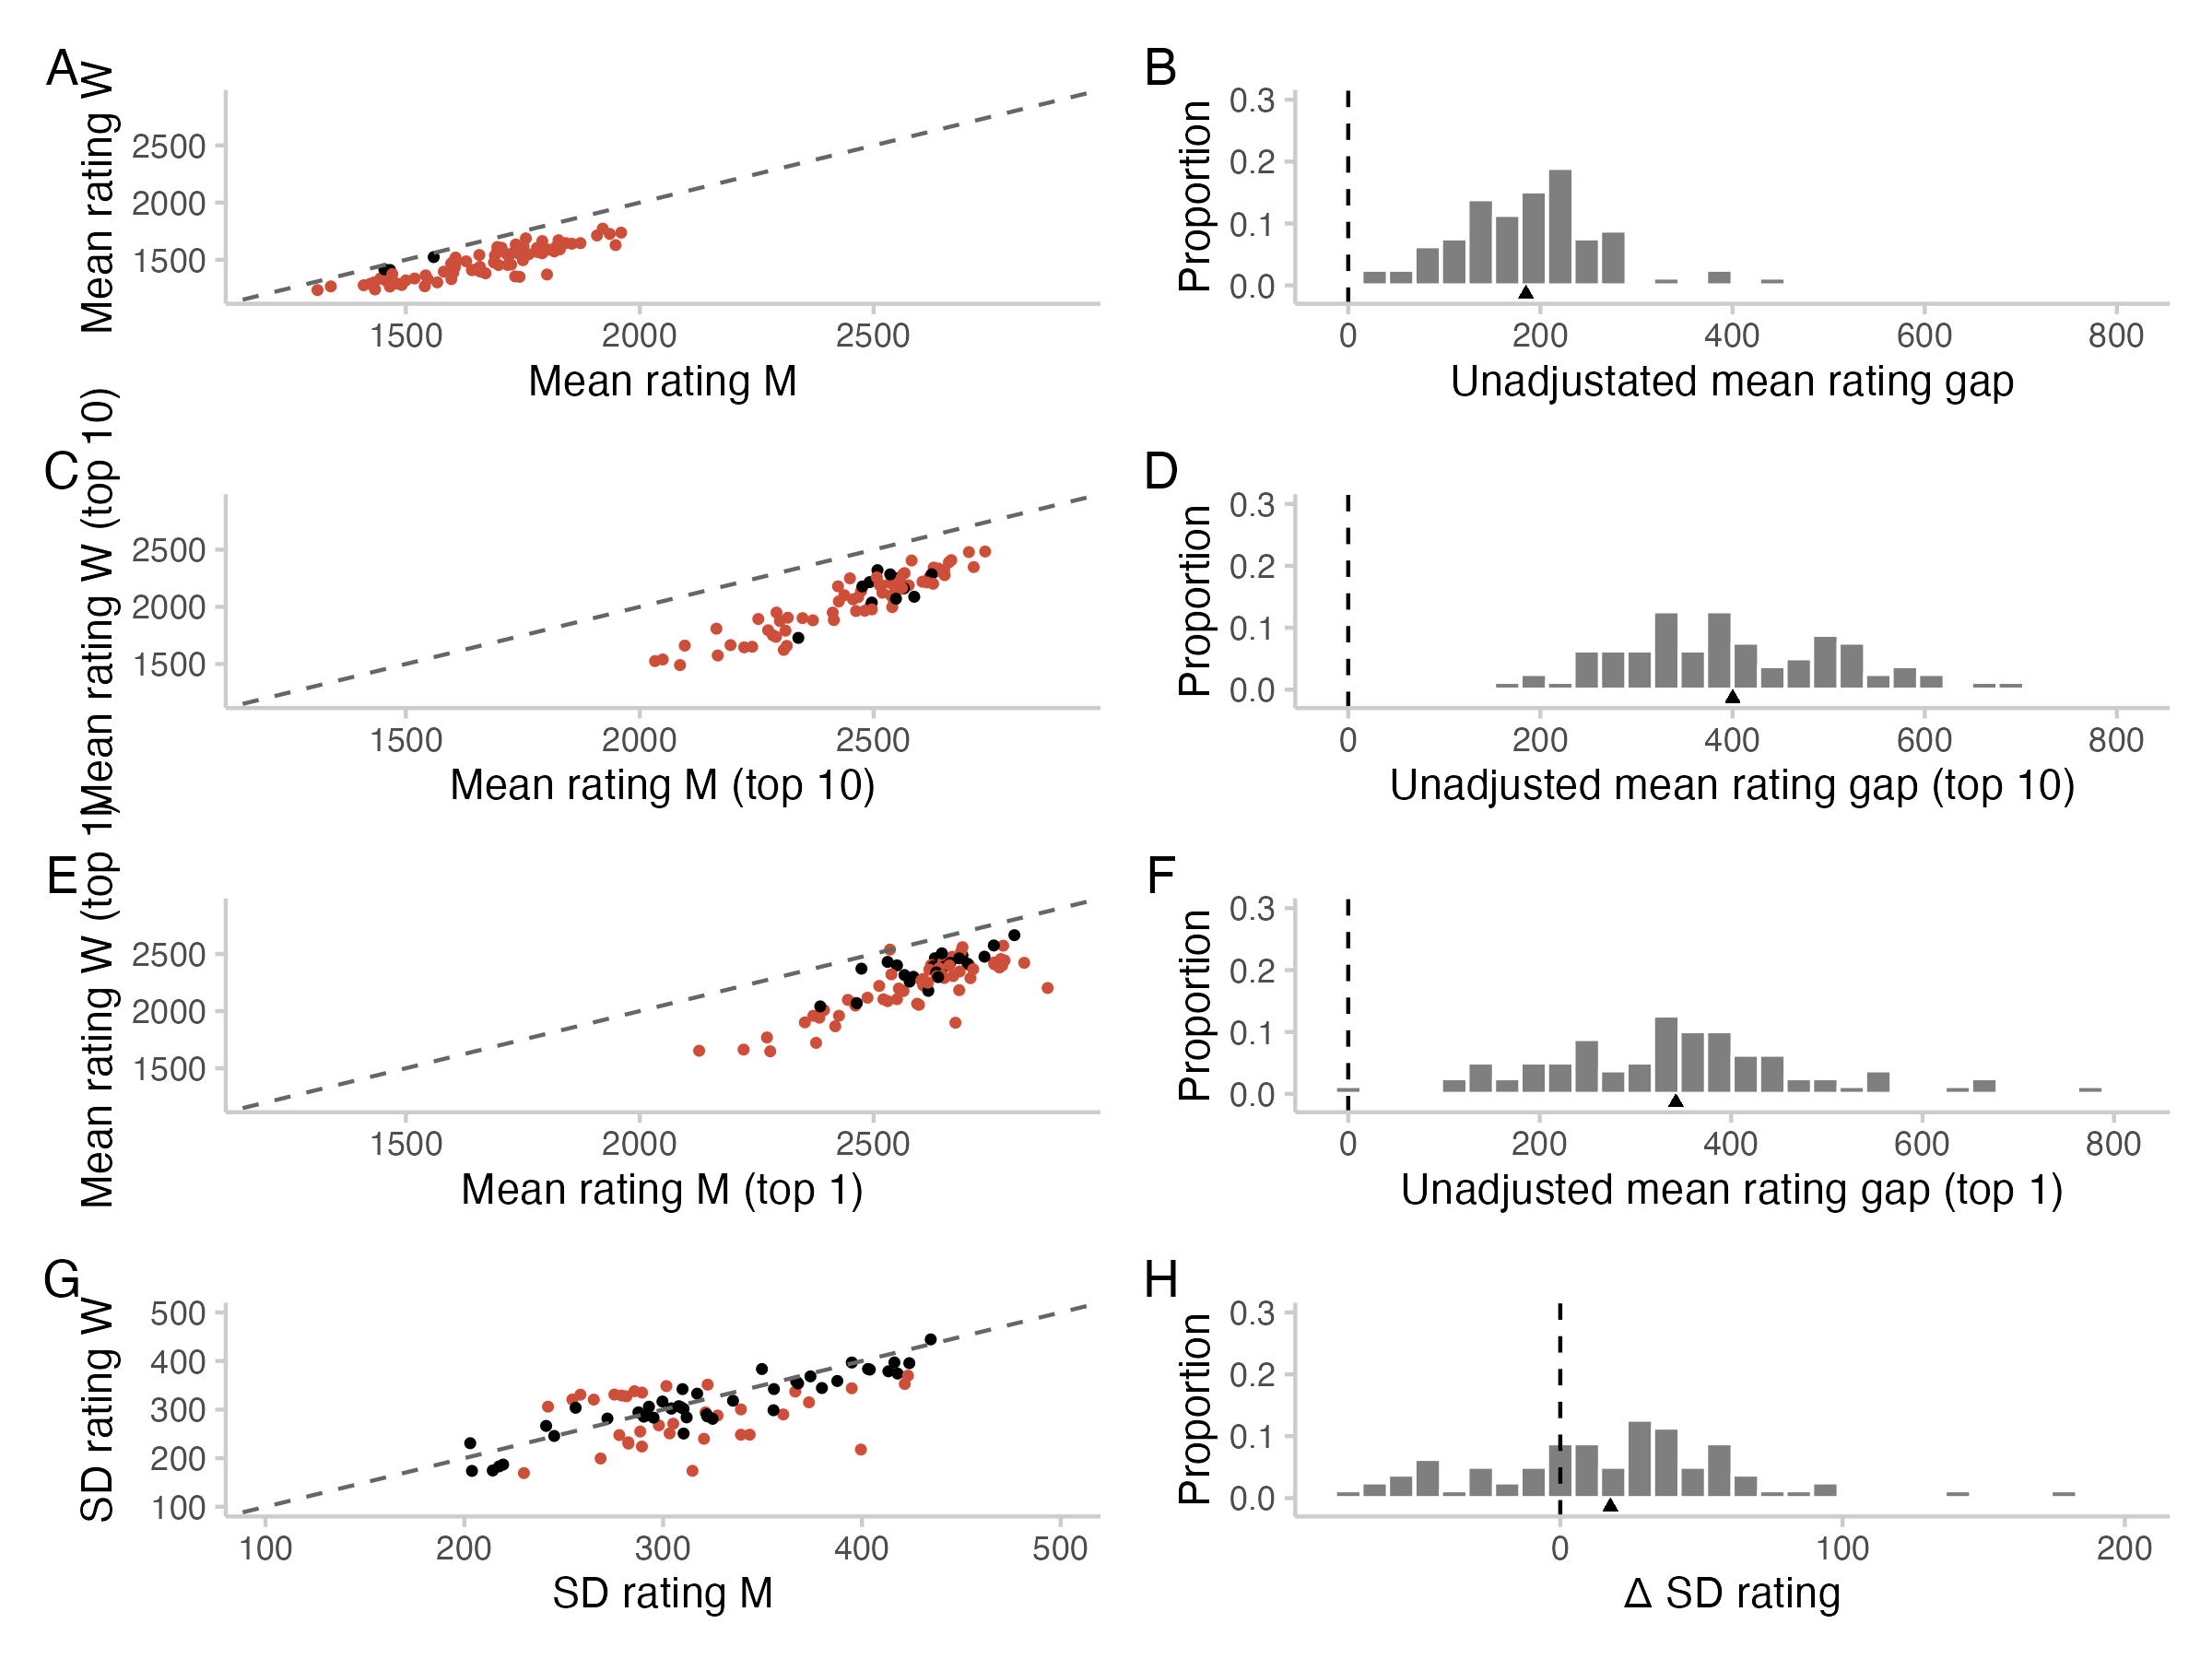
\includegraphics[width = \linewidth]{fig_2_w_jun_no_ina.png}
     \caption{Observed rating differences between men and women,  by federation. (A) Scatterplot of the mean rating of women against that of men. Each point represents a federation. Significant differences are marked in red. (B) Histogram of the difference in mean rating between women and men. (C-D) As (A-B) but for the mean rating of the top 10 players. (E-F) As (A-B) but for the top rating. (G-H) As (A-B) but for the standard deviation of rating.}.
     \label{fig:federation-differences}
 \end{figure}



\subsection*{Median}
The median rating of men was 1661, and of women 1381, for a difference of 280.  A permutation test revealed that this was significantly different from 0 ($p < 10^{-6}$). We next analyzed  median ratings by federation (Table \ref{tab:main_by_federation}).  In 78 out of 79 federations (all except Azerbaijan), men had a higher median median rating than women; out of those, the difference was significant in 67 federations (not in Armenia, Azerbaijan, Belarus, Bulgaria, China, Georgia, Kazakhstan, Latvia, Lithuania, Moldova, the United Arab Emirates, and Vietnam; also joined by Argentina after FDR correction). In the remaining federation (Azerbaijan), the difference was not significant. A KS test on the $p$-values revealed a distribution that was significantly different from uniform ($D=0.82$, $p < 10^{-15}$, both before and after FDR correction). We conclude that both in the aggregate and at the federation level, the median male rating is higher than the female rating.


\subsection*{Standard deviation and male variability hypothesis}
The {\it male variability hypothesis} states that men have more variance in cognitive abilities than women (CITE). We tested this hypothesis in our data set. Across the world, the rating SD of men was 349 and of women 333.5, for a difference of 15.5. This difference was significant (permutation test, $p < 10^{-6}$). We next analyzed rating standard deviations by federation (Fig. \ref{fig:federation-differences}D and Table \ref{tab:main_by_federation}). In 56 out of 79 federations, the SD was higher for men than for women. The difference was significant in 20 federations (12 after FDR correction) for men, and significant in 9 federations (5 after FDR correction) for women. A KS test on the $p$-values revealed a distribution that was significantly different from uniform ($D = 0.32$, $p = 1.8\times 10^{-7}$; after FDR correction: $D= 0.24$, $p=2\times 10^{-4}$). Thus, for a substantial fraction of federations, the difference between the rating SD of men and women is statistically significant, but the results are not all in the direction of greater variability among men.



\subsection*{Gender differences in the top ratings}
The main goal of this paper is to characterize and understand the gap in rating between top male and top women. It has been pointed out before that a difference in participation rate can contribute to a difference in the top gap \cite{charness1996participation, chabris2006sex, bilalic2009best}. Namely, the expected value of the maximum of i.i.d. variables  increases monotonically with the number of variables. Here, we offer a fresh approach to this question by estimating the sample distribution through permutations, separately for each federation. This allows us to determine how unexpected the observed top-level gap is given the participation gap, and to estimate the contribution of the participation gap to the top-level gap.

\subsection*{Top 1 gap}
 At the World level, the observed top 1 gap between men (Magnus Carlsen, rated 2872) and women (Hou Yifan, rated 2664) in our dataset was 208 Elo points. The expected gap is 87.3, which is $42\%$ of the observed gap. Based on a permutation test, we reject the null hypothesis that the top 1 gap can be fully accounted for by the participation gap ($p=2\times 10^{-4}$).  We next analyzed the top ratings by federation (Table \ref{tab:main_by_federation}). In 78 out of 79 federations (all but Lithuania), the highest rating among men was higher than among women. We reject the null hypothesis that the top 1 gap can be explained by the participation gap in 50 federations (34 after FDR correction). A KS test on the $p$-values revealed a distribution that was significantly different from uniform ($D=0.75$, $p < 2.2\times 10^{-16}$; after FDR correction: $D=0.73$, $p < 2.2\times 10^{-16}$). We conclude that both in the aggregate and at the federation level, the top rating of men is higher than that of women.

\subsection*{Top 10 gap}
For greater robustness, we repeated our analysis for the gap between the top 10 men and top 10 women players. At the World level, the observed top 10 gap between men (2790.0) and women (2561.0) was 229.0. The expected gap is 88.7, which is $38.7\%$ of the observed gap. Based on a permutation test, we reject the null hypothesis that the top 10 gap can be fully accounted for by the participation gap ($p < 10^{-6}$). We next analyzed the mean of the top 10 ratings by federation (Table \ref{tab:main_by_federation}). In all 79 federations, the mean of the top 10 ratings among men was higher than among women. Also in all federations, the observed top 10 gap was greater than the expected gap. We reject the null hypothesis that the top 10 gap can be explained by the participation gap in 65 out of 79 federations (63 after FDR correction). A KS test on the $p$-values revealed a distribution that was significantly different from uniform ($D=0.86$, $p < 2.2\times 10^{-16}$ both before and after FDR correction). Thus, the results for the mean of the top 10 ratings are qualitatively consistent with those for the top 1 rating.




\subsection*{Knapp rank analysis}
Knapp \cite{knapp2010prsb} proposed an alternative test based on ranks, which are arguably less informative than numerical ratings but the test is easier to compute, being based on one of the standard distributions of probability theory (hypergeometric). The results are qualitatively similar to those based on permutation tests. Details are in the Appendix.




\subsection*{P-adjusted gender gaps}
From here on, we focus on the three main gender gap metrics -- difference in overall mean rating, top 10 difference, and top 1 metrics.
For  any federation $i$ and any of these three metrics $y_i$, we denote by $\mu_i$ and $\sigma_i^2$ the mean and variance of the permutation null distribution of $y_i$. We call the difference between the actual difference and the expected difference if the participation rate hypothesis were correct, $y_i-\mu_i$, the {\it participation-adjusted} (P-adjusted) gender gap metric, and we will denote it by $y^\text{P}_i$. Fig. 3A-C show the distributions of the three P-adjusted gender gap metrics.


\begin{figure*}[!ht]
    \centering
        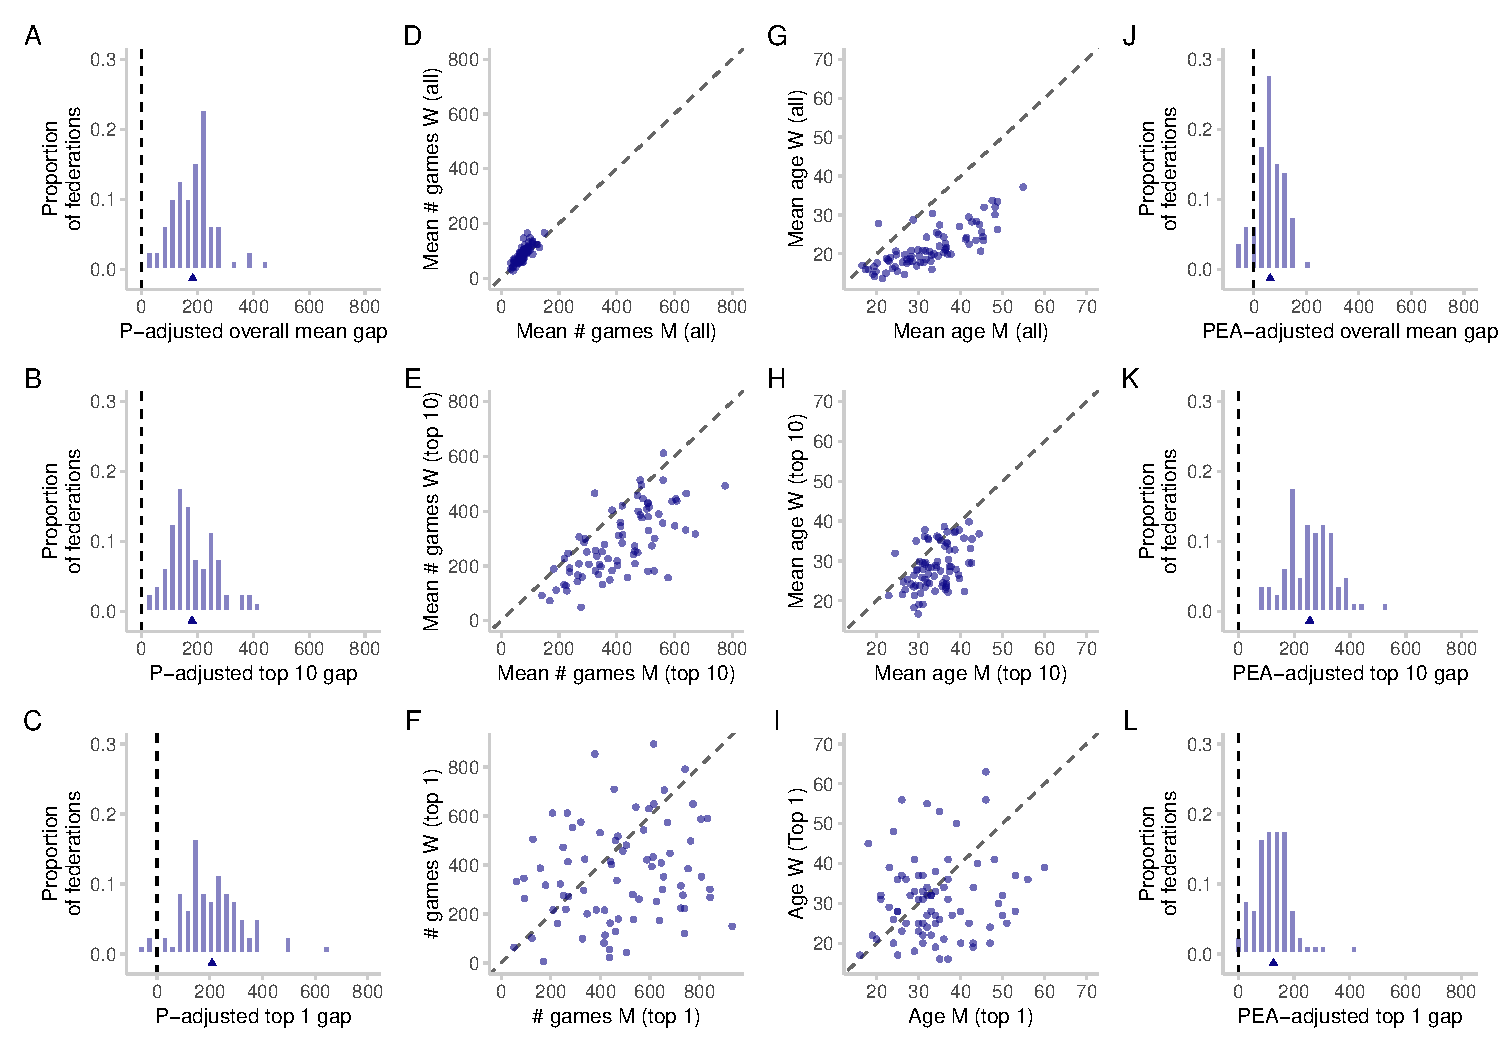
\includegraphics[width = \linewidth]{fig_3_w_jun_no_ina.pdf}
    \caption{Adjusting gender gaps for participation rate, experience, and age. We consider three difference metrics: between overall means, between top 10 means, and between the top 1 ratings. Each data point represents a federation. (A-C) Histograms of the P-adjusted metrics.
 The P-adjusted metric is the observed value minus the value expected under the null distribution used by a permutation test. Note that the overall mean does not need to be corrected for the participation gap. (D-F)  Experience comparisons between men and women players.  (G-I) Age comparisons between men and women players.  (J-K) Histograms of the PEA-adjusted metrics.
 The PEA-adjusted metric is the P-adjusted metric corrected for experience and age.}
    \label{fig:PEA}
\end{figure*}

\begin{table*}[t!]
\centering
\begin{tabular}{|c|c|c|c|c|c|c|c|c|c|c|}
\hline
\multirow{ 2}{*}{Metric} & \multicolumn{3}{c|}{Intercept, $w_0$} & \multicolumn{3}{c|}{Effect of experience, $w_E$} & \multicolumn{3}{c|}{Effect of age, $w_A$} \\
\cline{2-10}
  & Estimate & S.E. & $p$-value  & Estimate  & S.E. &   $p$-value  & Estimate  & S.E. &   $p$-value \\
\hline
Mean gap (All) & 100.0 & 14.5 & < 1e-8 & 1.96 & 0.45 & < 5e-5 & 7.84 & 1.12 & < 1e-9\\
\hline
Mean gap (Top 10) & 133.0 & 14.7 & < 1e-13 & 0.029 & 0.076 & 0.7 & 5.95 & 1.48 & < 2e-4\\
\hline
Gap (Top 1) & 185.0 & 13.6 & < 1e-21 & -0.034 & 0.045 & 0.45 & -1.02 & 0.93 & 0.28\\
\hline
\end{tabular}
\caption{Coefficients in a regression of P-adjusted gender gap metric against experience and age using the default data filter. See Supplementary Figure X for robustness.} \label{table:weighted-reg}
\end{table*}

\subsection*{Role of experience and age}
While a gender gap exists in most federations after correcting for the participation rate, we are specifically interested in cognitive, social, or biological factors contributing to this gap. Therefore, it is important to remove potential confounds of experience \cite{ de2022micro} and age \cite{smerdon2020female}. Computed by federation, men in our sample have more experience (Fig. 3D-F) and are older(Fig. 3G-I;\WJM{To create}) than women. These factors could contribute to men having higher ratings. Here, we correct for these confounds. We obtained age in years  by subtracting the player's birth year from 2019. We quantified experience as the total number of games played by each FIDE-rated player since October 2012, the earliest month for which rating data are available on the FIDE website. For each federation $i$, we denote by $y_i$ any of our three main P-adjusted gender gap metrics, $\Delta E_i$ the difference between the mean experience levels of the men and women used to calculate the gap metric, and by $\Delta A_i$ the corresponding age gap. We then fit the following regression model:
\begin{align}
    y^\text{P}_i = w_0 + w_E \Delta E_i + w_A \Delta A_i + \sigma_i \epsilon_i,
\end{align}
where $\epsilon_i$ denotes standard normal noise. Note that this is a heteroscedastic model: when the null distribution is wider, the P-adjusted gap metric is  noisier.  In the linear regression, this heteroscedasticity is taken into account by weighting the observations by the inverse variance, $\frac{1}{\sigma_i^2}$. The resulting coefficients are given in Table~\ref{table:weighted-reg}.


Indeed, differences in experience and age contribute to the P-adjusted gender gap. After estimating the coefficients, we define the gender gap metric adjusted for participation, experience, and age (PEA-adjusted), $y^\text{PEA}_i$, as
\begin{align}
 y^\text{PEA}_i & \equiv  y^\text{P}_i - \mu_i - \hat{w}_E \Delta E_i - \hat{w}_A \Delta A_i.
\end{align}
The mean PEA-adjusted gender gap is equal to the intercept $w_0$, i.e. \WJM{Mean and SEM needed here}. It is significantly different from 0 under all data filters (see Table 2), indicating that the gender gap remains after taking into account experience and age. However, it is much smaller in magnitude than the P-adjusted gap, let alone the gap in the raw data (for Top 10 and Top 1).  The distribution of the PEA-adjusted gender gap across federations is shown in Fig. 3J-L.


\subsection*{Robustness against changing the data filter}
We performed several robustness checks by varying the way we filter the data. Specifically, we explored the consequences of excluding junior players and/or including inactive players. We define a junior as a player with a birth year of 2000 or later, making them younger than 20 years old on Dec 31, 2019. Our methodology was otherwise the same. Tables \ref{tab:robustness_world} and \ref{tab:robustness_KS} show the results; details are in the Supplement. None of our statistical conclusions changes qualitatively, but excluding juniors reduces the number of federations for which the gap is significant.

\begin{table*}[t!]
\centering
\begin{tabular}{l|l|r|r|l|l|l|l|l}
\hline
Junior players & Inactive players & Rating floor & No. of federations & Mean & Median & SD & Top1 & Top10\\
\hline
No & No & 0 & 46 & 30 (26) & 24 (20) & 16 (10) & 15 (10) & 18 (10)\\
No & No & 1400 & 40 & 15 (10) & 13 (9) & 12 (5) & 13 (1) & 11 (8)\\
No & No & 1600 & 30 & 8 (6) & 8 (5) & 10 (6) & 11 (0) & 12 (8)\\
\hline
No & Yes & 0 & 77 & 59 (57) & 50 (45) & 31 (13) & 45 (37) & 61 (61)\\
No & Yes & 1400 & 69 & 44 (42) & 38 (29) & 34 (26) & 35 (25) & 51 (48)\\
No & Yes & 1600 & 62 & 31 (29) & 26 (17) & 31 (27) & 30 (23) & 40 (34)\\
\hline
Yes & No & 0 & 79 & 74 (74) & 67 (66) & 29 (17) & 50 (34) & 65 (63)\\
Yes & No & 1400 & 58 & 32 (26) & 31 (26) & 15 (12) & 22 (16) & 29 (18)\\
Yes & No & 1600 & 45 & 19 (15) & 16 (12) & 17 (11) & 18 (7) & 18 (13)\\
\hline
Yes & Yes & 0 & 99 & 93 (93) & 86 (86) & 40 (25) & 67 (65) & 91 (91)\\
Yes & Yes & 1400 & 79 & 58 (54) & 49 (47) & 40 (29) & 43 (38) & 60 (57)\\
Yes & Yes & 1600 & 65 & 42 (39) & 31 (25) & 41 (38) & 34 (30) & 48 (47)\\
\hline
\end{tabular}

\caption{Number of federations for which we reject the participation rate hypothesis, under various data filters. Filters are defined by whether junior players are included (first column), whether inactive players are included (second column), and whether there is a rating floor such that players below that rating are excluded from the analysis (third column). The fourth column shows the total number of federations with at least 30 players of each gender, after applying these filters. The rest of the columns show the number of federations for which we reject the participation rate hypothesis, with the column names indicating the summary metric over the ratings. In parentheses are the same numbers after applying the FDR correction.}
\label{tab:main_by_federation}
\end{table*}

\begin{figure*}[!ht]
  \centering
  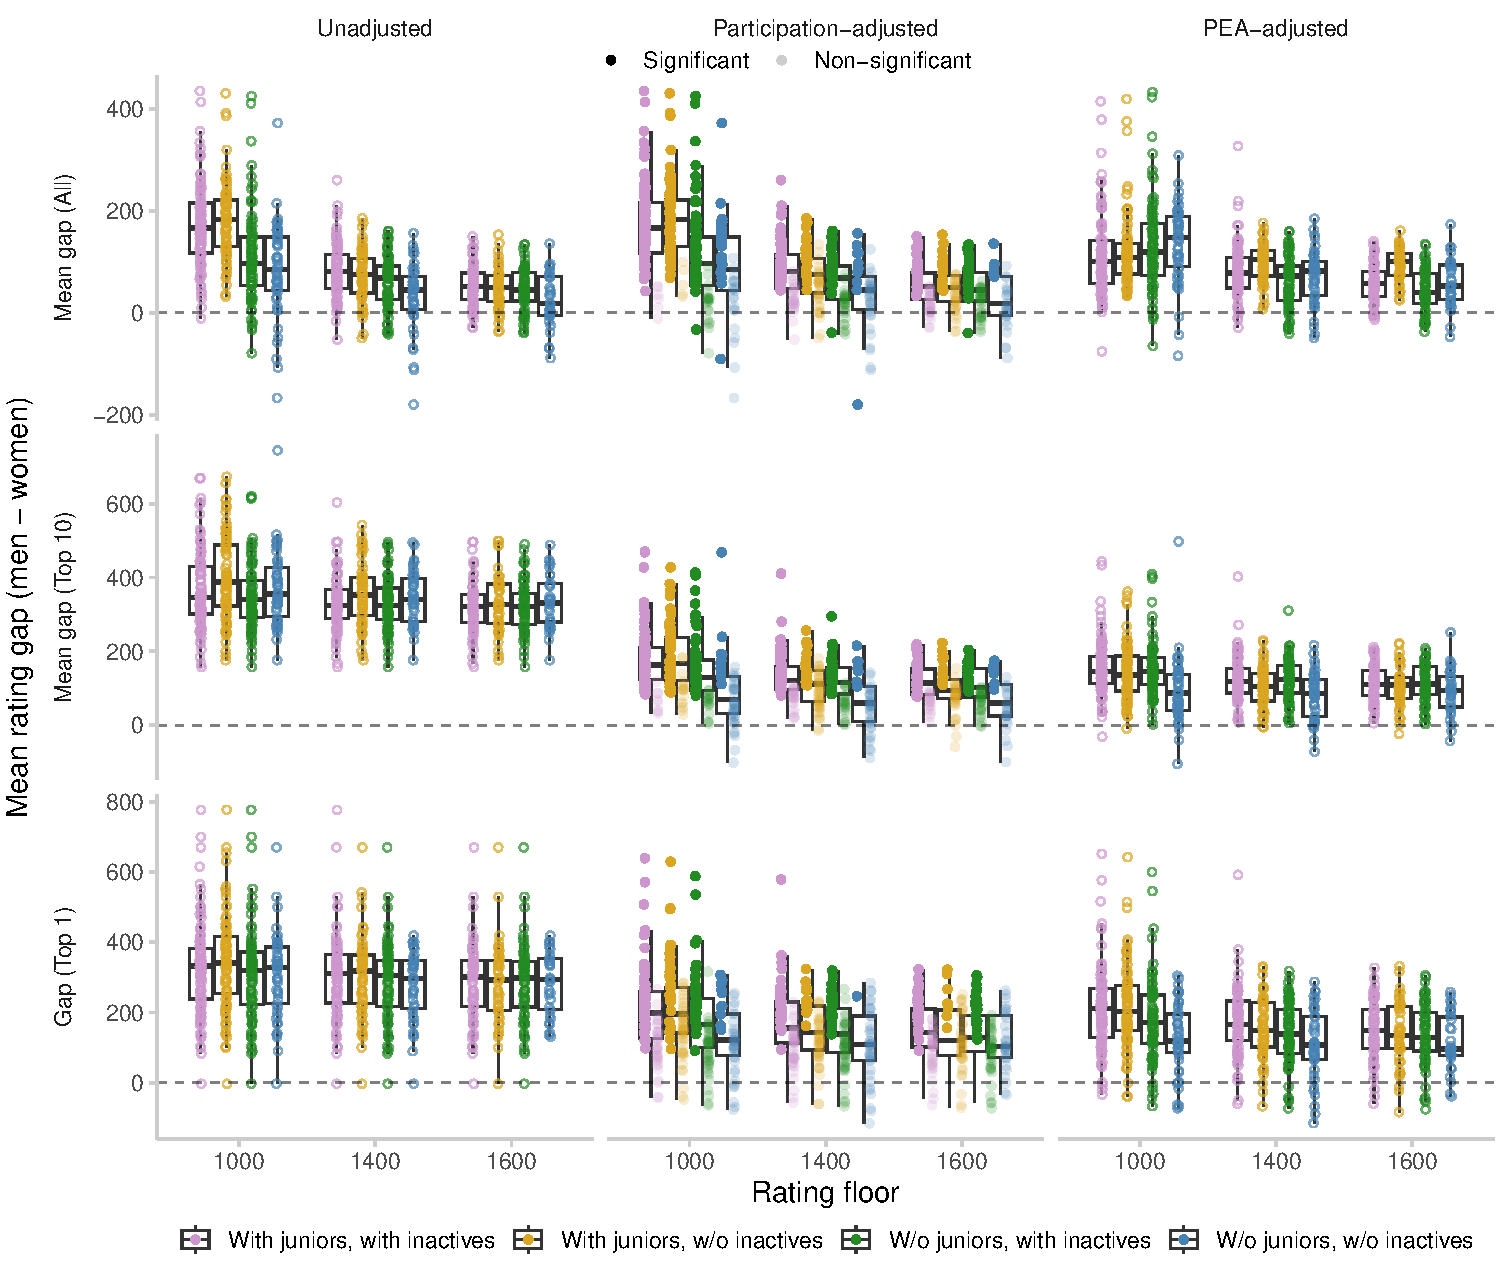
\includegraphics[width=\linewidth]{fig_4.pdf}
  \caption{Summary of the rating gap results, for all models and assumptions. Within each of the nine facets, the rating gap is along the y-axis, and the rating floor (the threshold below which players were excluded from the data) is along the x-axis. For each rating floor, four distributions of points are shown side by side. These correspond to additional data filters, showing all combinations of whether junior or inactive players are excluded from the data (colors). Each point is a single chess federation, with its y-coordinate showing the observed rating gap. The overall distribution of rating gaps is also summarized by box plots behind those points. The type of rating gap is shown in the facet rows, with the gap between the mean of all players (top row), the gap between the mean of the top ten players (middle), and the gap between top players (bottom) of each gender per federation. The facet columns refer to various statistical corrections applied to the ratings, with no correction (left column), participation-correction (middle), and participation-, experience-, and age-correction (PEA-correction; right). In the left and right columns, each federation is represented by an open circle. In the middle column each federation is a filled circle of high or low transparency (top legend below the label ``Participation-adjusted''), meaning that the corresponding rating gap is significant or non-significant under the participation rate hypothesis after False Discovery Rate-correction. The overall pattern is clear: uncorrected rating gaps are substantially larger than corrected ones. In addition, more restrictive data filters (both in terms of the rating floor and excluding junior/inactive players) lead to further diminished gaps. While the gender gap does not disappear, it is much smaller, and there are always federations where women are the stronger players.}
\end{figure*}


\section*{Discussion}

The results from our statistical analysis establish that a naive comparison of the observed top 1 (or top 10) gap as a metric for gender differences in chess performance leads to over-estimations of these differences, as it does not take into account the participation gap. However, when properly correcting for the gap, and also when considering mean and median ratings, we found that in most federations, as well as overall, women's chess ratings remain substantially lower than men's.

What could explain these remaining gaps? Popular opinions in the chess world can be classed along the familiar division of nature versus nurture. On one side, residual differences in playing strength may be attributed to biological, and in particular innate differences in ability or preferences, as publicly claimed by high-profile chess figures such as former World Champions Gary Kasparov and Bobby Fischer. On the other hand, the chess gender gap may be due to societal or cultural factors, a position supported by former top-10 player Judit Polgar and former World Champion Magnus Carlsen. In what follows, we outline the main classes of theories that could account for the remaining gap in performance, as well as potential explanations for the observed gap in participation. Dissecting their contributions is beyond the scope of this paper, so we consider this primarily a review and road map for future work.


%% TO EXPLAIN: GENDER GAPS IN CHESS PERFORMANCE
% - Participation gap itself
% - Residual top gap
% - Average gap in chess performance

%% POSSIBLE MEDIATING GENDER DIFFERENCES - EACH OF THESE COULD HAVE A BIOLOGICAL COMPONENT
% Gender differences in spatial cognition
% Gender differences in risk aversion and confidence
% Gender differences in competitiveness
% Gender differences in interest/preferences
% Gender differences in pressure/anxiety during play
% Gender differences in endurance

%% POSSIBLE SOCIAL/ENVIRONMENTAL FACTORS
% Home environment during childhood: Parental biases
% Chess community environment: Field-specific ability beliefs
% Chess community environment: Hostile environment
% Chess community environment: Stereotype threat
% Societal environment: Political system
% Societal environment: differences in prize money/national policies towards top players
% Home and societal environment: Family and child-rearing

\subsection*{Biological differences in ability}
A common argument for biological differences in chess ability is that chess involves visual-spatial thinking, and that men are innately better at that than women. Indeed, men tend to be better than women at visuospatial tasks \cite{kimura1999sex, terlecki2005important, voyer1995magnitude}, such as spatial attention and mental rotation.  Since chess ability relies heavily on spatial cognition, in particular pattern recognition and mental simulation (De Groot, Chase and Simon, Gobet), it is likely that gender differences in spatial cognition would translate to gender differences in chess ability.

There remains some debate about whether differences in spatial cognition are innate or acquired. A meta-analysis of gender differences in spatial cognition, in particular mental rotation, found that the magnitude of the advantage depends on age and that there might be no male advantage in early childhood \cite{lauer2019development}, thus challenging earlier claims that spatial cognition differences are innate. Parents speak to boys using more spatial terms than to girls, and a recent study found that this difference may fully explain the gap in spatial cognition observed between boys and girls by the age of 4 \cite{pruden2017}. In addition, the gender gap in spatial attention and mental rotation can be reduced by practicing action video games \cite{feng2007playing}, suggesting that experience plays an important role in the gap. In conclusion, open questions remain as to whether men are {\it innately} better than women in spatial cognition, as well as to what extent such spatial abilities predict chess ability.

\subsection*{Differences in interest and preferences}
Innate differences in interest may explain gender differences in participation, but the effect on the average performance level of a group is less clear. On the one hand, if girls are less interested in playing chess than boys, they might only continue playing chess if they are particularly good at chess, pushing up the relative average strength of women players. One other hand, lower interest may lead to girls putting in less effort and practice during their formative years, leading to less improvement and a lower relative average level. The latter mechanism could help account for the observed gender gap in strength after controlling for participation differences, while the former mechanism would go against it.

To our knowledge, no formal research has been conducted to explore gender differences in interest for chess. However, it is by now generally accepted that innate differences exist in terms of orientation towards `things' as opposed to `people' \cite{beltz2011,lippa2010}. Gender differences in preferences have been used to explain seemingly paradoxical cross-country results whereby countries with greater gender equality exhibit larger gender differences along several dimensions \cite{Falk2018,schmitt2017}, such as differences in STEM graduation \cite{Stoet2018}, though this literature is not without debate \cite{Richardson2020}. Recently, \citep{vishkin2022} reported a similar gender equality paradox with regard to chess participation, although the effect disappears when controlling for age differences and the main results conflict with similar analysis by \citep{dilmaghani2021}.

\subsection*{Differences in competitiveness}
A long history of research has found consistent differences between men and women in competitiveness. In laboratory experiments, women perform relatively worse than men in competitive environments compared to non-competitive environments, an effect that is stronger in mixed-sex competitions compared to single-sex competitions \cite{gneezy2003}, and women are roughly half as likely as men to select into competitive environments \cite{niederle2007}. The role of culture and institutions has been reported to play a large role in explaining the gap in competitiveness \cite{booth2018,zhang2018,andersen2013}, while there is mixed evidence for hormonal explanations \cite{apicella2011,wozniak2014,sapienza2009gender}. Additional evidence suggests that the gender gap in competitiveness already emerges at kindergarten age \cite{sutter2015} and widens towards extreme levels of competitiveness \cite{saccardo2018}. These results may explain the large gender-participation gap in competitive chess. However, as far as we know, no research has been carried out to examine whether there are gender differences in competitiveness among individuals who have \textit{already selected into} playing competitive chess, and recent research suggests that there are minimal or no gender differences in competitiveness among STEM professionals for this reason \cite{Boudreau2022}.



\subsection*{Field-specific ability beliefs}
Andrei Cimpian, Princeton University philosopher Sarah-Jane Leslie, and colleagues studied 30 academic disciplines in the U.S. and found a strong negative correlation between the pervasiveness of innate-ability beliefs and the proportion of female Ph.D.s. \cite{leslie2015expectations}. Moreover, very young children already internalize beliefs that men are more brilliant than women.

A 2017 study showed that 6-year-old girls in the U.S. are already less likely to believe that members of their gender are “really, really smart,” and that they begin avoiding activities that are said to be for children who are “really, really smart.” \cite{bian2017gender}. As chess is typically thought of as an activity for really smart people, it seems likely that early-life exposure to societal beliefs about intelligence contribute to the participation gap in chess.

Closely related to ability beliefs is the effect of stereotypes. Negative stereotypes about girls' performance potential in chess may lead both to drop-out and to lower performance for women who  continue to compete. A large number of studies have demonstrated that negative stereotypes about groups in cognitive domains may themselves be a cause of under-performance in those domains due to the pressure or anxiety induced by the stereotype. The `Stereotype Threat' effect has predominately been studied in the context of gender or racial differences in academic performance. Recent meta-analyses suggest that the stereotype threat causes females to perform worse on mathematical tests than males \cite{picho2013} and that interventions based around stereotype threat are largely effective \cite{liu2020}.

Stereotype threat has also been explored in the chess domain. Controlling for age and experience, \cite{smerdon2020female} show female tournament chess players underperform against male opponents relative to female opponents. The effect size is roughly equivalent to the disadvantage of playing with the black pieces in every game. \citep{maass2008} ran an experiment in which they manipulated whether or not subjects knew the gender of their opponents. Females performed worse when they believed they were playing against a male than when they believed they were facing another female, and lower chess-specific self-esteem was identified as a possible mechanism. These results are consistent with the gender composition differences in performance and competitiveness reported in \cite{gneezy2003}.

\subsection*{Parental and societal beliefs}
Parental beliefs are likely to also play a role. Parental influence may be affected by beliefs that girls are innately less good at some activities than others, or that chess is not a ``suitable" activity for girls. We have already discussed the role of parental use of spatial language as a factor in the development of gender differences in spatial cognition. Related to this, a well-known study reported that parents were three times more likely to explain science to boys than to girls at exhibits in a science museum \cite{crowley2001}. The authors found that the gender bias in parenting was likely not deliberate, but that this difference ``may be unintentionally contributing to a gender gap in children’s scientific literacy well before children encounter formal science instruction in grade school.''

Finally, there is some evidence that higher-level societal factors are associated with the gender-chess gap. In math -- a field much like chess in several ways -- a fascinating ``natural experiment'' took place when Germany split into East and West Germany. The gender gap in math ended up being much smaller in East than West Germany, arguably because the East's radically egalitarian system encouraged girls’ self-confidence and competitiveness in math \cite{lippmann2018math}. This demonstrates that gender differences in intellectual performance can be caused by society-level beliefs. Gender differences in competitiveness are smaller in (ex-)Communist federations \cite{zhang2018}, which may explain why the chess participation gap is smaller in `command economies' \cite{dilmaghani2021}.



\subsection*{Factors specific to top players}
In addition to the classes of arguments presented above, there are additional variables that may primarily explain differences among the very top chess players, and could be categorized to Objective and Subjective factors.
Monetary incentives is one of the essential objective factors that may favors men. Top prizes in Open section is typically two times higher compare to women-friendly events at different categories, including World Championship Match, Candidates Tournaments, World Cup and other world recognized Open Tournaments. Another existing factor that may cause the participation gap is the opportunities to accessing the top-level tournaments. Most of the elite chess events are only open to men participants, both because of the qualification system and inviting places that decides by ratings. Due to the phenomenon, the limited resources, such as technical support or training environment, that the local organization or government could provide for the players would also leaning towards men.
Reaching top-level chess requires a lot of inputs, such as training hours, pure concentration and other efforts which needs strong self- discipline. Due to general social value, it is much harder for women to keep professional training mode rather than men, as they were given various roles while they grow up. Therefore, the potential subjective factors could be explored further via Questionnaire or long-term follow-up. Another possible subjective factor is the willingness to fight during a game or a tournament. This could be done via statistical analysis.



\WJM{I am thinking we could use a simulation or calculation to show the effect of differences in top-level nurturing while accounting for base rates. Say we start with the same underlying distribution for men and women (but with fewer women), so that the residual top gap (observed minus expected) is zero. We then do an intervention that increases the ratings of both the top N men and the top N women, but more so for the men, then I think you will end up with a positive residual top gap. (Regardless of the fact that a woman gets paid more than a male player with the same rating.) This would show that the fact that a woman gets paid more than a male player with the same rating does not negate the possibility that differences in top-level nurturing help contribute to the observed top-level gap.}



\section*{Conclusion}
Statements by high-profile chess players, and occasionally by scientists \cite{howard2014jbs}, make it seem as if it is easy to  distinguish biological from non-biological factors; in reality, this is very hard. Conclusively establishing biological differences between genders is challenging for any cognitive ability, let alone for one that requires formal rules, such as chess. When children are old enough to be tested on such abilities, they have already been exposed to many social and environmental factors that could cause or contribute to gender differences.

It has been suggested that people are drawn to biological explanations because ``inherent explanations” serve to reinforce hierarchies \cite{hussak2015early}. That works out conveniently for those in high-status positions—who, in the chess world, tend to be men. It is harder to acknowledge that external factors, such as an unfair distribution of resources or a hostile environment, have held top women back.

We argue that there is a lack of research on social and environmental factors affecting women in chess, and that confidently attributing statistical differences to biological differences is a mistake.

\section*{Data}
Interactive data tool

\acknow{We thank Chessbase and Frederic Friedel.}

\showacknow{} % Display the acknowledgments section

% Bibliography
\bibliography{references}
\section*{Supporting Information}



\textbf{Hypergeometric distribution and Knapp's test}
\medskip

Suppose, within a single federation or overall, there are $N$ male players, $M$ female players, and the $K$'th best woman is ranked $R$ overall. In the following discussion, we treat $N,\ M$ and $K$ as fixed, and $R$ as a random variable.

Under the null hypothesis that the ranking order is random, we compute
\begin{eqnarray}
\Pr\{R=r\} & = & {{r-1 \choose K-1}{N+M-r\choose M-K}\over {N+M \choose M}}
\label{KT1}
\end{eqnarray}
provided $K\le r\le N+K$.

If the observed rank is $R=R^*$, then the one-sided p-value (probability of a result equal to or more extreme than that observed) is
\begin{eqnarray}
\sum_{r=R^*}^{N+K}\Pr\{R=r\}.
\label{KT2}
\end{eqnarray}

We computed [\ref{KT2}] for each federation as well as for the complete rating list. For example, in the complete rating list including juniors but excluding inactive players, we have $N=155368$, $M=17389$, and if $K=1$ then $R^*=79$ corresponding to Hou Yifan's rank as the top female player. Evaluating [\ref{KT1}] and [\ref{KT2}] in this case, $\Pr(R\ge 79)\approx 0.00025$ which we then interpret as the one-sided p-value under the participation rate hypothesis. When this analysis is repeated (with $K=1$) for the 79 individual federations, we find a statistically significant result ($p<0.05$) in 56 federations, going up to 65 or 64 respectively if $K=10$ or $K=30$ (recall that the criterion for a federation being included is that it should have at least 30 female players). If instead we base the calculation on two-sided p-values, the numbers of statistically significant results are respectively 51, 58, 59 for $K=1,\ 10,\ 30$. However interpreted, these results show that the participation rate hypothesis is rejected for the vast majority of federations. This test is effectively equivalent to Knapp's test \cite{knapp2010prsb} and has the merit of being an exact calculation not requiring simulation.

\medskip
\textbf{Tables}

\medskip

\onecolumn


\begin{center}
\begin{tabular}{|l|l|}
\hline
 FED  &  Three-letter abbreviation for federation\\
Obs1  &  Observed difference between top 1 male and female ratings \\
Mean1  &  Expected difference between top 1 male and female ratings \\
PV1    &  p-value based on top 1 male and female ratings \\
Obs10  &  Observed difference between top 10 male and female ratings \\
Mean10  &  Expected difference between top 10 male and female ratings \\
PV10    &  p-value based on top 10 male and female ratings \\
Obsall  &  Observed difference between overall mean male and female ratings \\
Meanall  &  Expected difference between overall mean male and female ratings \\
PVall    &  p-value based on overall mean male and female ratings \\
Knapp1 & p-value under Knapp test with $k=1$\\
Knapp10 & p-value under Knapp test with $k=10$\\
Knapp30 & p-value under Knapp test with $k=30$\\
\hline
\end{tabular}
\end{center}
\vskip0.2in
\hskip0.5in
\textbf{\large Supplementary Table 2: Explanation of columns in Supplementary Table 1.}

\newpage

\begin{table*}[t]
\caption{Like Table 1 but for different data filters.}
\end{table*}




\end{document}


